\documentclass[../main.tex]{subfiles}
\graphicspath{{\subfix{../IMAGES/}}}


\begin{document}
\localtableofcontents

Heat transfer is thermal energy in transit. It happens when there is a temperature difference. Three ways : \begin{itemize}
    \item Conduction : heat flows within solids (or stationary fluids) \begin{equation}
        q" = -\kappa \frac{dT}{dx}
    \end{equation}\\
    \item Convection : heat flows between a moving fluid and a solid \begin{equation}
        q" = \overline{h} (T_s-T_\infty)
    \end{equation}\\
    \item Radiation : heat flows without a medium \begin{equation}
        Q_{rad} = \varepsilon \sigma A_s (T^4-T_{sur}^4)
    \end{equation} with $\sigma = 5.67\cdot 10^{-8}$ [J/s m$^2$ k$^4$], the Stefan-Boltzmann constant\\
\end{itemize}

\quad \underline{Closed system :} No mass flow across the boundary\\

\begin{equation}\begin{gathered}
    \Delta U = Q-W + E_{gen} [J]\\
    \Dot{U} = \dot{Q}-\dot{W}+ \Dot{E}_{gen} [W]\\
    \end{gathered}
\end{equation}

With : \begin{itemize}
    \item $Q \begin{cases}
        > 0 & \text{enters the system}\\
        <0 & \text{exits the system}\\
    \end{cases}$\\
    \item $W \begin{cases}
        > 0 &\text{done BY the system}\\
        <0 &\text{done ONTO the system}\\
    \end{cases}$\\
    \item $E_{gen}\begin{cases}
        > 0 &\text{heat released}\\
        < 0 &\text{heat absorbed}\\
    \end{cases}$
\end{itemize}

Control volume encompasses only the interface and has no mass, no thermal capacity, no work and no sources. Therefore : $0 = \sum Q$\\

\quad \underline{Open system :} advection of energy must be included\\

\begin{equation}
    \begin{gathered}
        \Dot{E}_{stored} = \Dot{E}_{in} - \Dot{E}_{out} + \Dot{E}_{gen} \\
        = \dot{m} (u+pv + \frac{1}{2}V^2+gz)_{in} - \dot{m} (u+pv + \frac{1}{2}V^2+gz)_{out} +Q - W\\
    \end{gathered}
\end{equation}

\quad \underline{Ideal gas :}\\
\begin{itemize}
    \item Change in enthalpy : $h_{in}-h_{out} = c_p (T_{in}-T_{out})$(h=u+pv)\\
    \item Change in internal energy : $u_{in}-u_{out} = c_v (T_{in}-T_{out})$\\
\end{itemize}

\begin{equation}
    \frac{dE_{st}}{dt} = \dot{U} = mc_v \frac{dT}{dt} = Q-W+\dot{E}_{gen}
\end{equation}


Incompressible fluid : $c_p = c_v$\\

\quad \underline{Inequality of Clausius :}\\
Whenever a system undergoes a cycle, the integral around the cycle of $\frac{dQ}{T}$ is less than zero for an irreversible cycle and equal to zero for a reversible cycle or : $\int \frac{dQ}{T}\leq 0 \Rightarrow dS = \frac{dQ}{T}$, with S the entropy.\\

Real processes are irreversible. We need transport laws to determine the heat flux.\\

\begin{itemize}
    \item Q : heat transfer rate [W]\\
    \item q" : heat flux [W/m$^2$]\\
    \item q' : heat flux unit length [W/m]\\
    \item $\dot{q}$ : volumetric heat source [W/m$^3$]\\
\end{itemize}

\subsection{Fourier's law and heat conduction}

\begin{equation}
\begin{gathered}
    q" = -\kappa \frac{dT}{dx}\\
    \Vec{q}" = -\kappa \nabla T\\
    \end{gathered}
\end{equation}

With $\kappa$ the thermal conductivity [W/mK].\\
Heat flux is perpendicular to the isothermal surface. 

If the material is anisotropic : $\Vec{q}" = -\overline{\overline{\kappa}} \nabla T$, with $\overline{\overline{\kappa}} = \begin{pmatrix}
    k_x & 0 & 0\\
    0 & k_y & 0\\
    0 & 0 & k_z\\
\end{pmatrix}$\\

Assumptions : \begin{enumerate}
    \item incompressible medium\\
    \item medium at rest (no convection)\\
    \item isotropic material\\
\end{enumerate}


The energy conservation equation requires : \begin{equation}
    \dot{U} = mc\frac{dT}{dt} = Q+\dot{E}_{gen}
\end{equation}

Heat transfer rate OUT of dS : $\delta Q = (-\kappa \nabla T)\cdot (\Vec{n}dS)$\\

Total heat transfer rate INTO non-isothermal S : $Q = -\int_S (-\kappa \nabla T)\cdot (\Vec{n} dS)$\\
Total generation rate in volume : $\dot{E}_{gen} = \int_V \dot{q}dV$\\
Change in internal energy of the volume : $\frac{dU}{dt} = \int_V \rho c \frac{\partial T}{\partial t}dV$\\

\begin{equation}
    \begin{gathered}
        \dot{U} = Q + \dot{E}_{gen}\\
        \Rightarrow 0 = \int_V (\nabla \cdot (\kappa \nabla T) + \dot{q} - \rho c \frac{\partial T}{\partial t})dV\\
        \nabla \cdot (\kappa \nabla T) + \dot{q} = \rho c \frac{\partial T}{\partial t}\\
        \nabla^2 T + \frac{\dot{q}}{\kappa} = \frac{1}{\alpha} \frac{\partial T}{\partial t}\\
        \alpha = \frac{\kappa}{\rho c}\\
    \end{gathered}
\end{equation}
With $\alpha$ the thermal diffusivity [$m^2$/s]\\

The higher the thermal conductivity and the lower the thermal capacity, the higher the material diffusivity.\\

\subsubsection{Solution of equation}
We here assume three more things : \begin{itemize}
    \item $\kappa$ is independent of T\\
    \item steady-state ($\frac{\partial}{\partial t}=0$)\\
    \item no heat sources ($\dot{q}$ = 0)\\
\end{itemize}

These assumptions lead to : $\nabla^2 T = 0$\\
\warning We need Boundary Conditions !\\

\begin{itemize}
    \item Cartesian coordinates : $\frac{\partial^2 T}{\partial x^2} + \frac{\partial^2 T}{\partial y^2} + \frac{\partial^2 T}{\partial z^2} = 0$\\
    \item Cylindrical coordinates : $\frac{1}{r} \frac{\partial}{\partial r}(\kappa r \frac{\partial T}{\partial r}) + \frac{1}{r^2} \frac{\partial}{\partial \varphi} (\kappa \frac{\partial T}{\partial \varphi}) + \frac{\partial}{\partial z}(\kappa \frac{\partial T}{\partial z}) = 0$\\
\end{itemize}

Assume that either Temperature only depends on x or equivalently on r : \begin{itemize}
    \item Cartesian : \begin{equation}
        \frac{\partial T^2}{\partial x^2} = 0 \Rightarrow T(x) = C_1x + C_2
    \end{equation}
    \item Cylindrical : \begin{equation}\frac{1}{r} \frac{\partial}{\partial r}(\kappa r \frac{\partial T}{\partial r}) = 0 \Rightarrow C_1 \ln(r) + C_2 \end{equation}\\
\end{itemize}

Three kinds of boundary conditions : \begin{enumerate}
    \item Dirichlet condition (constant surface temperature) : $T(\Vec{r}) = T_w$\\
    \item Neumann condition (known heat flux) : $-\kappa(\frac{\partial T}{\partial x})_{x=x_i} = q"_w$ (if $q"_w = 0$, then we have an adiabatic wall or symmetry plane)\\
    \item Robin condition (convection surface condition) : $-\kappa (\frac{\partial T}{\partial x})_{x_i} = h(T(x_i,t)-T_\infty)$\\
\end{enumerate}

Example for planar wall in 1D : \begin{itemize}
    \item Temperature boundary condition : $T(x) = \frac{T_2-T_1}{L}x+T_1$, $Q = -\kappa A \frac{T_2-T_1}{L}$ 
    \item constant heat flux and temperature : $T(x) = -\frac{q_1"}{\kappa} (x-L) + T_2$, $Q = Aq_1"$\\
    \item constant heat flux and convection : $T(x) = -\frac{q_1"}{\kappa}(x-L) + \frac{q_1"}{h} + T_\infty$, $Q = Aq_1" = Aq_2"$\\
\end{itemize}

\warning In a planar wall, temperature profile is always LINEAR. If no heat source inside the wall, the heat flux has to be equal on each side of the domain.\\

Example for a temperature boundary condition in a pipe : $T(r) = \frac{T_1-T_2}{\ln(\frac{r_1}{r_2})} \ln(\frac{r}{r_2}) + T_2$, $Q = \frac{2\pi L \kappa}{\ln(\frac{r_2}{r_1})}(T_1-T_2)$\\


\subsubsection{Thermal resistance}
The higher the thermal conductivity, the lower the thermal resistance, the lower the temperature drop.\\

For a planar wall : \begin{itemize}
    \item Conduction : $R_{th} = \frac{L}{\kappa A}$\\
    \item Convection : $R_{th} = \frac{1}{hA}$\\
    \item Radiation : $R_{th} = \frac{1}{h_{rad} A}$\\
\end{itemize}

For a cylindrical system : \begin{itemize}
    \item Conduction : $R_{th} = \frac{\ln(\frac{r_2}{r_1})}{2\pi L\kappa}$\\
    \item Convection : $R_{th} = \frac{1}{h 2\pi r L}$\\
    \item Radiation : $\frac{1}{h_{rad} 2\pi r L}$\\
\end{itemize}

With for the radiation : $Q = A \varepsilon \sigma (T_s^2 + T_{sur}^2)(T_s+T_{sur})(T_s-T_{sur}) = A h_{rad}(T_s-T_{sur})$\\

In a circuit, we can apply the rule : $R_{series} = \sum R_i$ and compute the heat flux from the boundary by taking the total thermal resistance of the circuit.\\

Finally, we can define the \textbf{Biot number} : \begin{equation}
    Bi = \frac{R_{th,cond}}{R_{th, conv}} = \frac{hL}{\kappa}
\end{equation}
\warning $L = \frac{V}{A_s}$ a characteristic dimension\\

We have three cases : \begin{enumerate}
    \item Bi << 1 : solid has approximately a constant temperature\\
    \item Bi$\simeq$1 : convection decreases the temperature as much as conduction\\
    \item Bi>>1 : convection does not play an important role in heat loss\\
\end{enumerate}

\quad \underline{Overall Heat Transfer Coefficient :}\\

\begin{equation}
    \begin{gathered}
        U = \frac{1}{R_{tot}A} = \frac{1}{R"_{tot}}\\
        Q_x = UA(T_1-T_4)\\
    \end{gathered}
\end{equation}

\warning UA is a constant of the system. If the area is not constant, U depends on the position.\\

\subsubsection{With heat sources}
\begin{equation}
    \nabla^2T + \frac{\dot{q}}{\kappa} = \frac{1}{\alpha} \frac{\partial T}{\partial t}
\end{equation}

We have five assumptions : \begin{enumerate}
    \item incompressible medium\\
    \item medium at rest (no convection)\\
    \item isotropic material\\
    \item $\kappa$ is independent of T\\
    \item \textbf{steady-state}\\
\end{enumerate}

The equation now becomes : $\nabla^2T + \frac{\dot{q}}{\kappa} = 0$\\

\begin{itemize}
    \item Cartesian : \begin{equation}
        T(x) = -\frac{\dot{q}}{2\kappa}x^2 + C_1 x + C_2
    \end{equation}
    \item cylindrical : \begin{equation}
        T(r) = -\frac{\dot{q}}{4\kappa}r^2 + C_1\ln(r) + C_2
    \end{equation}
\end{itemize}

\quad \underline{1D, Cartesian coordinates :}\\

If we apply temperature boundary condition : $T(x=-L) = T_1$, $T(x=L)=T_2$\\
We get a \textbf{PARABOLIC} T(x) profile : $T(x) = \frac{\dot{q}}{2\kappa}L^2(1-\frac{x^2}{L^2})+\frac{T_2-T_1}{2} \frac{x}{L} + \frac{T_1+T_2}{2}$\\

With the position of the maximum being : $x_{max} = \frac{\kappa}{\dot{q}} \frac{T_2-T_1}{2L}$\\

$Q = -\kappa A \frac{\partial T}{\partial x} = Q(x)$ \warning It is not constant!\\

\warning We cannot use the thermal resistance concept in layers with heat sources\\

The heat transfer rate follows the temperature gradient. The heat generated on the right of $x_{max}$ will flow towards the right surface and vice-versa.\\

if $T_1 = T_2$, at the centerline of the wall the heat flux is zero. This is equivalent to having a perfectly insulated boundary at $x=0$.\\

\quad \underline{1D, cylindrical coordinates :}\\

We impose a temperature boundary condition at the surface $T(r_0)= T_s$\\
We also need to satisfy a symmetry condition $\frac{dT}{dr}\lvert_{r=0}=0$\\

We get $T(r)= \frac{\dot{q}r_0^2}{4\kappa}(1-\frac{r^2}{r_0^2})+T_s$\\

\subsubsection{2D conduction}

We use here the principle of separation of variables : 
\begin{equation}
    \begin{gathered}
        \frac{\partial^2 T}{\partial x^2} + \frac{\partial^2 T}{\partial y^2} = 0\\
        \theta = \frac{T-T_1}{T_2-T_1}\\
        \theta(x,y) = X(x)Y(y) \Rightarrow -\frac{1}{X} \frac{d^2X}{dx^2} = \frac{1}{Y} \frac{d^2Y}{dy^2}\\
    \end{gathered}
\end{equation}

Finally, we get : 

\begin{equation}
    \theta = (C_1\cos(\lambda x) + C_2\sin(\lambda x))(C_3 e^{-\lambda y} + C_4 e^{\lambda y})
\end{equation}

\subsubsection{Shape factor for known heat diffusion problems}

For numerous geometries an analytical solution has been found and can be retrieved using a \textbf{Shape factor S} : 
\begin{equation}
    Q = kS(T_1-T_2)
\end{equation}

\begin{table}[hbt!]
    \centering
    \begin{tabular}{c|c}
        System & Shape factor S\\
        \hline
        Isothermal sphere buried in a semi-infinite medium & $\frac{2\pi D}{1-\frac{D}{4z}}$ \\
        Horizontal isothermal cylinder of length L buried in a semi-infinite medium & $\frac{2\pi L}{\cosh^{-1}(\frac{2 z}{D})}$\\
        Vertical cylinder in a semi-infinite medium & $\frac{2\pi L}{\ln(\frac{4L}{D})}$\\
        Conduction between two cylinders of length L in infinite medium & $\frac{2\pi L}{\cosh^{-1}(\frac{4w^2-D_1^2-D_2^2}{2D_1D_2})}$\\
    \end{tabular}

\end{table}

\subsection{Extended surfaces (fins)}

If we take a generalized fin (area not constant), we can define two surfaces :\begin{itemize}
    \item $A_c = A_c(x)$ the cross-section of the fin\\
    \item $dA_s = P(x)dx$, with $A_s$ the external surface and $P(x)$ the perimeter on the infinitesimal surface\\
\end{itemize}

From Energy Balance, we get $Q_x = Q_{x+dx} + dQ_{cond}$\\
Which can be rewritten as : \begin{equation}
    \frac{d^2T}{dx^2} + (\frac{1}{A_c} \frac{dA_c}{dx})\frac{dT}{dx} - (\frac{h}{A_c \kappa} \frac{dA_s}{dx}) (T-T_\infty) = 0
\end{equation}

\warning We assumed here no heat sources !\\

If we further assume a constant cross-section, we get : \begin{equation}
    \begin{gathered}
        \frac{d^2T}{dx^2} - \frac{hP}{A_c \kappa} (T-T_\infty) = 0\\
        \Theta = \frac{T-T_\infty}{T_b-T_\infty}\\
        \xi = \frac{x}{L}\\
        m^2 = \frac{hP}{\kappa A_c}\\
        \Rightarrow \frac{d^2 \Theta}{d \xi^2} - (mL)^2 \Theta = 0\\
    \end{gathered}
\end{equation}

Also, we can see that $(mL)^2 = \frac{(L/\kappa A_c)}{1/hPL} \simeq \frac{R_{cond}}{R_{conv}}$\\

\begin{itemize}
    \item If $(mL)^2>>1$, fin has added a large thermal resistance\\
    \item If $(mL)^2<<1$, fin has added little surface area\\
    \item A good fin will have a value around 1 to balance internal and external resistance\\
\end{itemize}

The total heat removed by the fin is then : $Q_{fin} = Q_{b,cond} = -\kappa A \frac{d\theta}{dx}\lvert_{x=0}$\\

We can define different types of boundary conditions : \begin{itemize}
    \item Fin base : $T = T_b$, $\Theta_{\xi=0} = 1$\\
    \item Fin tip : \begin{enumerate}
        \item Adiabatic : $\frac{d\Theta}{d\xi}\lvert_{\xi = 1} =0$\\
        \item Convection : $\Theta_{\xi=1} = h A_c (T(L)-T_\infty)$\\
        \item Temperature : $\Theta_{\xi=1} = \Theta_L$\\
        \item Infinite fin : $\Theta_L \rightarrow 0$\\
    \end{enumerate}
\end{itemize}

\begin{table}[hbt!]
    \centering
    \begin{tabular}{c|c|c|c}
        Case & Tip condition (x=L) & Temperature distribution $\frac{\theta}{\theta_b}$ & Fin heat transfer rate $Q_f$\\
        \hline
        A & Convection heat transfer : $h \theta(L) = -\kappa \frac{d\theta}{dx}\lvert_{x=L}$ & $\frac{\cosh m(L-x) + (h/m\kappa) \sinh m(L-x)}{\cosh mL + (h/m\kappa) \sinh mL}$ & $M \frac{\sinh mL + (h/m\kappa) \cosh mL}{\cosh mL + (h/m\kappa) \sinh mL}$\\
        B & Adiabatic $\frac{d\theta}{dx}\lvert_{x=L} = 0$ & $\frac{\cosh m(L-x)}{\cosh mL}$ & $M \tanh mL$\\
        C & Prescribed temperature $\theta(L) = \theta_L$ & $\frac{(\theta_L/\theta_b) \sinh mx + \sinh m(L-x)}{\sinh mL}$ & $M\frac{(\cosh mL-\theta_L/\theta_b)}{\sinh mL}$\\
        D & Infinite fin $(L\rightarrow \infty)$ $\theta(L)=0$ & $e^{-mx}$ & $M$\\
    \end{tabular}
\end{table}

With $M = \sqrt{hP\kappa A_c} \theta_b$\\

We can now define some useful metrics : \begin{itemize}
    \item Fin efficiency : 
    \begin{equation}
        \eta_f = \frac{Q_f}{hA_f(T_b-T_\infty)}
    \end{equation}
    with $A_f$ the external area for convection. Fin efficiency is useful to estimate $Q_f$\\
    \item Fin effectiveness : \begin{equation}
    \varepsilon_f = \frac{Q_f}{h A_{c,b}(T_b-T_\infty)} = \frac{R_{conv,b}}{R_f} = \frac{1/hA_{c,b}}{1/h\eta_f A_f}
    \end{equation}
    It is the ratio between the heat transfer with fin and without. We can also make a resistance for the fin : $R_f = \frac{1}{h \eta_f A_f}$\\
    To be useful, the fin must have a combined thermal resistance $R_f$ lower than the convection resistance of the base $R_{conv,b}$\\
\end{itemize}

\begin{table}[hbt!]
    \centering
    \begin{tabular}{c|c}
        Straight fins & $\eta_f = \frac{\tanh mL_c}{mL_c}$ \\
        Triangular & $\eta_f = \frac{1}{mL} \frac{I_1(2mL)}{I_0(2mL)}$\\
        Parabolic & $\eta_f = \frac{2}{[4(mL)^2 + 1]^{\frac{1}{2}}+1}$\\
        Circular fin & $\eta_f = C_2 \frac{K_1(mr_1) I_1(mr_{2c}) - I_1(mr_1) K_1(mr_{2c})}{I_0(mr_1)K_1(mr_{2c}) + K_0 (mr_1) I_1(mr_{2c})}$\\
        Pin fins & $\eta_f = \frac{\tanh mL_c}{mL_c}$\\
    \end{tabular}
\end{table}

\subsubsection{Fin arrays}
We mostly utilize an array of fins rather than a single fin.\\
Let $A_b$ be the exposed surface without fins. We have the thermal resistance $R_{Nf} = \frac{1}{Nh \eta_f A_f}$\\

The performance can be measured with $\eta_t = 1-\frac{NA_f}{A_t} (1-\eta_f)$ which leads to $R_t = \frac{1}{\eta_t h A_t}$\\

\subsection{Transient heat diffusion}

\subsubsection{Uniform Temperature in the solid}
We need here $\kappa$ high enough and Bi<<1 (Bi<0.1)\\

We also assume that the liquid temperature remains constant at all times.\\

\begin{equation}
    \begin{gathered}
        0 = -Q_{cond}-W+\dot{E}_{gen} - mc \frac{dT}{dt}\\
        T(t) = (T_i-T_\infty) e^{-\frac{hA_s}{\rho Vc}t}+ T_\infty\\
        \frac{\theta}{\theta_i} = e^{-\frac{1}{R_{conv}C_{th}}t}\\
        C_{th} = \rho Vc\\
        R_{conv} = \frac{1}{h A_s}\\
    \end{gathered}
\end{equation}


We call this analogy the \textbf{lumped capacitance model}.\\

We get the total heat removed : $Q[J] = \int_0^t Q_{conv} dt = \rho Vc \theta_i [1-e^{-\frac{t}{\tau_{th}}}]$\\

We can also define \textbf{Fourier number} : \begin{equation}
    Fo = \frac{\alpha t}{L^2}
\end{equation}
With $\alpha = \frac{\kappa}{\rho c}$\\

Therefore we have : $\frac{\theta}{\theta_i} = e^{-Bi\cdot Fo}$\\

\begin{figure}[hbt!]
    \centering
    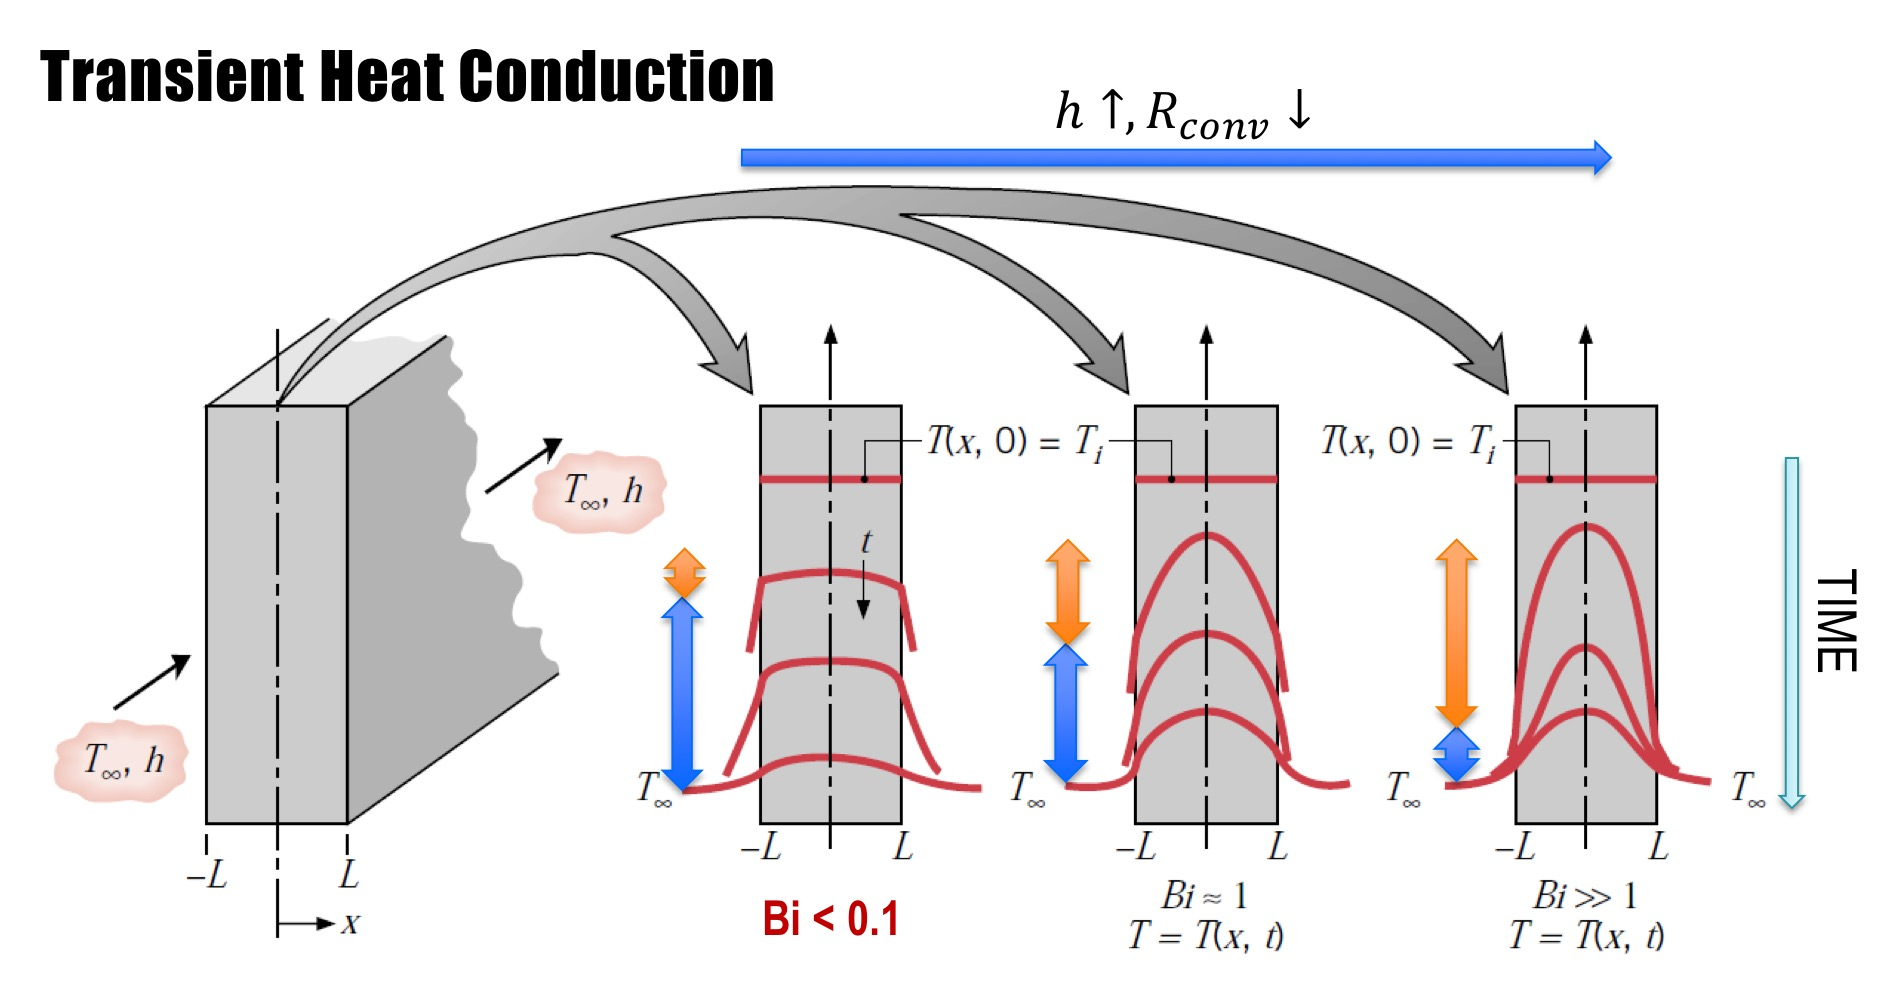
\includegraphics[width = .6\textwidth]{IMAGES/elec/IMG_0165.jpeg}
\end{figure}

\subsubsection{Bi>0.1}

Let's define : \begin{itemize}
    \item $\theta^* = \frac{\theta}{\theta_i}$\\
    \item $x^* = \frac{x}{L}$
\end{itemize}

\begin{equation}
    \begin{gathered}
        \frac{\partial^2 \theta^*}{\partial x^{*2}}\\
        \theta^* (x^*,0)=1\\
        \frac{\partial \theta^*}{\partial x^*}\lvert_{x^* = 1} = -Bi \theta^*(1,t^*)\\
        \frac{\partial \theta^*}{\partial x^*} \lvert_{x^* = 0} = 0\\
    \end{gathered}
\end{equation}

For which we have the solution : \begin{equation}
    \theta^* = \sum_n A_n exp(-\lambda_n^2 Fo)\cos(\lambda_n x^*/L)
\end{equation}

\warning If Fo > 0.2, the first harmonic dominates : \begin{equation}
    \theta^* = A_1 exp(-\lambda_1^2 Fo) \cos(\frac{\lambda_1 x}{L})
\end{equation}

The total heat removed is now : $\frac{Q}{Q_0} = 1-D_1 exp(-\lambda_1^2 Fo)$\\

For Bi>0.1 and Fo>0.2, we have the following : \begin{itemize}
    \item Planar Wall $\theta^* = A_1 exp(-\lambda_1^2 Fo) \cos(\frac{\lambda_1 x}{L}) = \theta_0 \cos(\frac{\lambda_1 x}{L})$, $\theta_0$ the temperature evolution at the center of the slab. $Fo = \frac{\alpha t}{L^2}$, $Bi = \frac{hL}{\kappa}$, $\frac{Q}{Q_0} = 1-\frac{\sin \lambda_1}{\lambda_1} \theta_0$ \warning L is the half thickness of the layer\\
    \item Cylinder $\theta^* = A_1 exp(-\lambda_1^2 Fo) J_0 (\frac{\lambda_1 r}{r_0}) = \theta_0 J_0 (\frac{\lambda_1 r}{r_0}$, $Fo = \frac{\alpha t}{r_0^2}$, $Bi = \frac{h r_0}{\kappa}$, $\frac{Q}{Q_0} = 1-\frac{2}{\lambda_1}\theta_0 J_1 (\lambda_1)$\\
    \item Sphere $\theta^* = A_1 exp(-\lambda_1^2 Fo) \frac{r_0}{\lambda_1 r} \sin(\frac{\lambda_1 r}{r_0}) = \theta_0 \frac{r_0}{\lambda_1 r} \sin(\frac{\lambda_1 r}{r_0})$, $Fo = \frac{\alpha t}{r_0^2}$, $Bi = \frac{h r_0}{\kappa}$, $\frac{Q}{Q_0} = 1-\frac{3}{\lambda_1^3} \theta_0 [\sin(\lambda_1) - \lambda_1 \cos(\lambda_1)]$\\
\end{itemize}

Bi number : \begin{table}[hbt!]
    \centering
    \begin{tabular}{c|c|c|c}
         & Square & Cylinder & Sphere \\
         \hline 
        Lumped Capacitance Model & $\frac{h2t}{\kappa}$ & $\frac{h r_0}{2\kappa}$ & $\frac{h r_0}{3\kappa}$\\
        Bi > 0.1 & $\frac{ht}{\kappa}$ & $\frac{h r_0}{\kappa}$ & $\frac{h r_0}{\kappa}$\\
    \end{tabular}
\end{table}


\subsubsection{Semi-infinite Wall (1D)}
We have $T(x\rightarrow \infty, t) = T_i$\\

We introduce a similarity variable $\eta$ : \begin{equation}
    \eta = \frac{x}{\sqrt{4 \alpha t}}
\end{equation}

\begin{equation}
    \frac{\partial^2 T}{\partial \eta^2} = -2\eta \frac{\partial T}{\partial \eta}
\end{equation}

We have three cases : \begin{enumerate}
    \item $T(x,0) = T_i$, $T(0,t) = T_s$ \begin{equation}
        \frac{T(x,t) - T_s}{T_i-T_s} = erf(\frac{x}{2\sqrt{\alpha t}})
    \end{equation}
    \item $T(x,0) = T_i$, $-\kappa \frac{\partial T}{\partial x}\lvert_{x=0} = q_0"$ \begin{equation}
        T(x,t) - T_i = \frac{2 q_0" (\alpha t/ \pi)^{\frac{1}{2}}}{\kappa} exp(\frac{-x^2}{4 \alpha t}) - \frac{q_0" x}{\kappa} erfc(\frac{x}{2\sqrt{\alpha t}})
    \end{equation}
    \item $T(x,0) = T_i$, $-\kappa \frac{\partial T}{\partial x}\lvert_{x=0} = h[T_\infty - T(0,t)]$ \begin{equation}
        \frac{T(x,t) - T_i}{T_\infty - T_i} = erfc(\frac{x}{2\sqrt{\alpha t}}) - [exp(\frac{h x}{\kappa} + \frac{h^2 \alpha t}{\kappa^2})] [erfc(\frac{x}{2\sqrt{\alpha t}} + \frac{h \sqrt{\alpha t}}{\kappa})]
    \end{equation}
\end{enumerate}

In the first case, we also get $q_s" = \frac{\kappa (T_s-T_i)}{\sqrt{\pi \alpha t}}$\\

\subsubsection{Periodic Heating}
We have $T(0,t) = T_i + \Delta T \sin(\omega t)$\\

\begin{equation}
    \begin{gathered}
        \frac{T(x,t) - T_i}{\Delta T} = exp[-x \sqrt{\frac{\omega}{2\alpha}}] \sin[\omega t - x\sqrt{\frac{\omega}{2\alpha}}]\\
        q_s"(t) = \kappa \Delta T \sqrt{\frac{\omega}{\alpha}} \sin(\omega t + \frac{\pi}{4})\\
    \end{gathered}
\end{equation}

\subsection{Convection}
We have four kinds of convection : \begin{enumerate}
    \item Forced convection\\
    \item Natural convection\\
    \item Boiling \\
    \item Condensation\\
\end{enumerate}

It refers to the heat transfer between a solid and a fluid in motion when they are at different temperature.\\
During convection, heat is transferred through diffusion and advection.\\

\subsubsection{Fluid dynamics}
For Newtonian fluids, we have $\tau(\overline{y}) = \mu \frac{\partial u}{\partial y}\lvert_{y=\overline{y}}$ and at the wall : $\tau(0) = C_f \frac{\rho u_\infty^2}{2}$\\

Conservation of mass : $\frac{\partial \rho u}{\partial x} + \frac{\partial \rho v}{\partial y} = 0$\\

Conservation of momentum : $u \frac{\partial u}{\partial x} + v \frac{\partial u}{\partial y} = -\frac{1}{\rho} \frac{\partial p}{\partial x} + v\frac{\partial^2 u}{\partial y^2}$\\

The Bernoulli equation for the free flow is : $\frac{p}{\rho} + \frac{u_\infty^2}{2} = cste$\\

We can make the equations dimensionless : $u = -\frac{\partial \psi}{\partial y}\lvert_x$, $v = -\frac{\partial \psi}{\partial x}\lvert_y$ ($\psi$ a streamline).\\

$\eta = y \sqrt{\frac{u_\infty}{v x}}$, $f(\eta) = \frac{\psi}{u_\infty \sqrt{\frac{vx}{u_\infty}}}$\\
\warning For laminar flow only
\begin{equation}
    \begin{gathered}
        2 \frac{d^3f}{d\eta^3} + f \frac{d^2 f}{d\eta^2} = 0\\
        \frac{u}{u_\infty} = \frac{df}{d\eta}\\
        \tau(0) = \mu u_\infty \frac{\sqrt{u_\infty}}{\sqrt{vx}} \frac{d^2 f}{d\eta^2}\lvert_{\eta = 0}\\
        \tau_x = C_f(x) \rho u_\infty^2/2\\
        C_f(x) = \frac{0.664}{\sqrt{Re_x}} \text{ (at boundary layer)}\\
    \end{gathered}
\end{equation}




We have the thickness of the boundary layer : $\frac{\delta}{x} = \frac{4.92}{\sqrt{Re_x}}$, $Re_x = \frac{u_\infty x}{v}$\\

Finally, the velocity distribution in the boundary layer is defined as : \begin{equation}
    v = 0.5 (\frac{\nu u_\infty}{x})^{1/2} [\eta f'(\eta)-f]
\end{equation}

\subsubsection{Convection coefficient}
At the wall, the velocity is zero : $q"(0) = -\kappa_f \frac{\partial T}{\partial y}\lvert_{y=0}$\\

\begin{equation}
    h = \frac{-\kappa_f \frac{\partial T}{\partial y}\lvert_{y=0}}{(T_s-T_\infty)}
\end{equation}

At the boundary layer, we have the temperature $T_\infty$.\\
Let $L_c$ be a characteristic dimension of the problem : \begin{equation}
    \frac{h L_c}{\kappa_f} = \frac{\partial (\frac{T_s-T}{T_s-T_\infty})}{\partial (\frac{y}{L_c})}\lvert_{y/L_c = 0} = N u_L
\end{equation}
With $Nu_L$ the Nussel number.\\

The temperature gradient at the wall changes as the temperature boundary layer develops. \textbf{The convection coefficient varies spatially} : $\overline{h} = \frac{1}{A_s} \int h dA_s$ the average convection coefficient.\\

As we are in open system, we have $\dot{U} = \dot{m}(u+pv+\frac{1}{2}V^2 + gz)_{in} - \dot{m} (u+pv + \frac{1}{2}V^2 + gz)_{out} + \dot{Q} - \dot{W} + \dot{E}_{gen}$ but as the control volume does not move, we have $\dot{U} = -(\rho \Vec{u}\cdot \Vec{n}) (h) + \dot{Q} + \dot{E}_{gen}$ : \begin{equation}
    \int_V \frac{\partial \rho u}{\partial t}dR = -\int_S (\rho h \Vec{u})\cdot (\Vec{n} dS) - \int_S (-\kappa \nabla T)\cdot(\Vec{n}dS) + \int_V \dot{q}dR
\end{equation}

We need to make 6 assumptions : \begin{enumerate}
    \item isotropic material\\
    \item potential and kinetic energy changes are negligible\\
    \item neglect the effect of pressure changes dp on enthalpy, internal energy and density\\
    \item density changes result only from temperatures changes so the fluid is incompressible $\nabla \cdot \Vec{u} = 0$\\
    \item all material parameters are temperature independent\\
    \item viscous stresses do not dissipate enough energy to warm the fluid\\
\end{enumerate}

\begin{equation}
    \rho c_p(\frac{\partial T}{\partial t} + \Vec{u}\cdot \nabla T) = \kappa \nabla^2 T + \dot{q}
\end{equation}

Let the dimensionless parameter be : $x^* = \frac{x}{L}$, $y^* = \frac{y}{L}$, $u^* = \frac{u}{u_\infty}$, $v^* = \frac{v}{u_\infty}$, $p^* = \frac{p}{\rho u_\infty^2}$, $T^* = \frac{T-T_s}{T_\infty-T_s}$\\

\begin{itemize}
    \item Navier-Stokes : $u^* \frac{\partial u^*}{\partial x^*} + v^* \frac{\partial u^*}{\partial y^*} = -\frac{\partial p^*}{\partial x^*} + \frac{1}{Re_L} \frac{\partial^2 u^*}{\partial y^{*2}}$\\
    \item Energy conservation : $u^* \frac{\partial T^*}{\partial x^*} + v^* \frac{\partial T^*}{\partial y^*} = \frac{1}{Re_L Pr} \frac{\partial^2 T^*}{\partial y^{*2}}$\\
\end{itemize}

With $Pr = \frac{\text{kinematic diffusivity}}{\text{heat diffusivity}} = \frac{\nu}{\alpha_f} = \frac{\mu c_{p,f}}{\kappa_f} = \frac{\delta}{\delta_t}$ the \textbf{Prandtl number}\\
Where $\delta$ is the thickness of the velocity boundary layer and $\delta_t$ of the temperature.\\
\warning We need to use the fluid properties not the solid ones!\\

If Pr<<1, heat diffuses very quickly relative to momentum.\\

\quad \underline{Pr = 1 :}\\
We have $\delta(x) = \delta_t(x)$\\
$h = \kappa_f \frac{\sqrt{u_\infty}}{\sqrt{vx}} f"\lvert_{\eta=0}$\\

From the table, we get $\frac{hx}{\kappa_f} = 0.332 \sqrt{Re_x}$\\

Also, $C_f = \frac{0.664}{\sqrt{Re_x}}$\\

We therefore get : \begin{table}[hbt!]
    \centering
    \begin{tabular}{c|c|c|c}
    Local coefficients & $\tau_w = 0.332 \frac{\mu u_\infty}{x} \sqrt{Re_x}$ & $C_f = \frac{0.664}{\sqrt{Re_x}}$ & $\frac{hx}{\kappa_f} = Nu_x = 0.332 Re_x^{1/2} Pr^{1/3}$\\
    \hline
     Average coefficients & $\tau_w = 0.664 \frac{\mu u_\infty}{x}\sqrt{Re_x}$ & $\overline{C}_f = \frac{1.328}{\sqrt{Re_x}}$ & $\frac{\overline{h}x}{\kappa_f} = \overline{Nu}_x = 0.664 Re_x^{1/2} Pr^{1/3}$  \\
    \end{tabular}
\end{table}


\begin{itemize}
    \item BL of a flat plate in parallel flow : \begin{itemize}
        \item if laminar $Nu_x = .332 Re_x^{1/2} Pr^{1/3}$ and $\overline{Nu}_x = 0.664 Re_x^{1/2} Pr^{1/3}$ (Pr>0.6)\\
        \item else $Nu_x = 0.0296 Re_x^{4/5} Pr^{1/3}$ and $\overline{Nu}_x = 0.037 Re_x^{4/5} Pr^{1/3}$ (0.6<Pr<60)\\
    \end{itemize}
    \item Cross-flow around a cylinder : $\overline{Nu}_D = 0.3 + \frac{0.62Re_D^{1/2} Pr^{1/3}}{[1+(0.4/Pr)^{2/3}]^{1/4}} [1+(\frac{Re_D}{282000})^{5/8}]^{4/5}$, $Re_D = \frac{u_\infty D}{\nu}$\\
    \item Bank of tubes : \begin{itemize}
        \item Aligned (separated by $S_T$ and $S_L$) : $V_{max} = \frac{S_T}{S_T-D}V$\\
        \item Staggered (diagonal $S_D$) : \begin{enumerate}
            \item if $S_D = [S_L^2 + \frac{S_T^2}{4}]^{1/2} > \frac{S_T + D}{2}$, then $V_{max} = \frac{S_T}{S_T-D}V$\\
            \item else $V_{max} = \frac{S_T}{2(S_D-D)}V$\\
        \end{enumerate}
        We have $Re_{D,max} = \frac{\rho V_{max}D}{\mu}$ ($N_L \geq 20$, $0.7<Pr<500$, $1000<Re_D<2e6$) $\overline{Nu}_D = C_2 C Re_D^mPr^{0.36} (\frac{Pr}{Pr_s})^{1/4}$ ($Pr_s$ the prandtl estimated at the temperature of the outer surface of the tubes) : \begin{equation}
            \begin{gathered}
                \Delta T_{lm} = \frac{(T_s-T_i) - (T_s - T_0)}{\ln(\frac{T_s-T_i}{T_s-T_0})}\\
                \frac{T_s-T_0}{T_s-T_i} = e^{-\frac{\pi D N\overline{h}}{\rho V N_T S_T c_p}}\\
                q' = N(\overline{h} \pi D \Delta T_{lm})\\
            \end{gathered}
        \end{equation}
    \end{itemize}
\end{itemize}


\textbf{The generalized form of the convection coefficient : } \begin{equation}
    Nu_x = CRe_x^a Pr^b
\end{equation}

\warning Flow is considered laminar if $Re < 5e5$\\



\subsubsection{Internal flows}
In a pipe, after a distance $x_{fd,h}$ or entrance length, we get an entirely viscous flow ($\tau \neq 0$). It is a \textbf{fully developed flow}.\\

In a pipe, we consider two states : \begin{itemize}
    \item Laminar flow : $Re_D<2300$ and $(\frac{x_{fd,h}}{D}) \simeq 0.05 Re_D$\\
    \item Turbulent flow : $Re_D>2300$ and $10<(\frac{x_{fd,h}}{D})<60$ \\
    \item $Re_D = \frac{\rho u_m D}{\mu}$, $u_m$ mean velocity\\
\end{itemize}

For a circular tube : $u_m = \frac{4\dot{m}}{\rho \pi D^2}$, $Re_D = \frac{4\dot{m}}{\pi D\mu}$\\

In this region we have a poiseuille flow and therefore : $\frac{u(r)}{u_m} = 2[1-(\frac{r}{r_0})^2]$\\
We have : $C_f = \frac{f}{4}$, $f$ the friction (Darcy) factor\\
\begin{itemize}
    \item $f = \frac{64}{Re_D}$\\
    \item for smooth surfaces a good correlation is : $f = (0.79 \ln Re_D-1.64)^{-2}$\\
\end{itemize}

\quad \underline{Thermal aspects :}\\
We have two possible boundary conditions : heat flux $q"_s$ and temperature $T_s$\\

\begin{itemize}
    \item Temperature fixed at wall : The temperature of the fluid will continue to increase approaching $T_s$. As the temperatures become more similar the heat flux will decrease and $\frac{\partial T}{\partial r}\lvert_{r=r_0}$ decreases along x.\\
    \item The heat flux is fixed. $\frac{\partial T}{\partial r}\lvert_{r=r_0}$ is constant along x. \\
\end{itemize}

Contrary to the velocity profile $u(r)$, $T(x,r)$ continues to change with x even when the thermal boundary layers have merged.\\

We need to define the fully developed region : \begin{equation}
    \begin{gathered}
        \theta = \frac{T_s(x) - T(r,x)}{T_s(x) - T_m(x)}\\
        \frac{\partial \theta}{\partial x}\lvert_{x = x_{fd,t}} = 0\\
    \end{gathered}
\end{equation}

\warning In the fully developed region h is constant\\

We have the mean temperature described as : \begin{equation}
    T_m = \frac{2}{u_m r_0^2} \int_0^{r_0} u Trdr
\end{equation}

The global energy balance is defined as : \begin{equation}
    Q_{conv} = \dot{m} c_p(T_{m,o}-T_{m,i})
\end{equation}

The local energy balance can be written as : \begin{equation}
    \frac{dT_m}{dx} = \frac{q_s"P}{\dot{m}c_p} = \frac{P}{\dot{m}c_p} h(T_s-T_m)
\end{equation}

With P the perimeter of the pipe.\\

We need boundary conditions to solve : \begin{itemize}
    \item Constant Heat Flux BC ($q_s"$) : \begin{equation}
    \begin{gathered}
        T_m(x) = \frac{q_s" P}{\dot{m}c_p}x + T_{m,i}\\
        Q_{conv} = q_s" Pdx\\
        \end{gathered}
    \end{equation}
    \item Constant Temperature BC ($T_s$) : \begin{equation}\begin{gathered}
        \frac{T_s-T_{m,0}}{T_s-T_{m,i}} = e^{-\frac{PL \overline{h}}{\dot{m}c_p}}\\
        Q_{conv} = \overline{h} A \Delta T_{lm}\\
        \Delta T_{lm} = \frac{\Delta T_0-\Delta T_i}{\ln(\frac{\Delta T_0}{\Delta T_i})}\\
        \end{gathered}
    \end{equation}
\end{itemize}
In order to maintain a constant wall temperature, we might want to do a convection on the pipe. By doing so, we change $T_s$ with temperature of the fluid $T_\infty$ and we need to use the total equivalent resistance.\\

For an open system, we have assuming we are in the fully developed region and with a laminar flow : \begin{equation}
    u \frac{\partial T}{\partial x} = \frac{\alpha}{r} \frac{\partial}{\partial r} (r\frac{\partial T}{\partial r})
\end{equation}

Two types of boundary conditions : \begin{itemize}
    \item Constant heat flux : \begin{equation} \begin{gathered}
        T(r,x) = T_s(x) - \frac{2u_m r_0^2}{\alpha} (\frac{dT_m}{dx}) [\frac{3}{16} + \frac{1}{16}(\frac{r}{r_0})^4 - \frac{1}{4} (\frac{r}{r_0})^2]\\
        h = \frac{48}{11} \frac{\kappa_f}{2r_0}\\
        Nu_D = \frac{hD}{\kappa_f} = 4.36\\
        \end{gathered}
    \end{equation}\\
    \item Constant $T_s$ : \begin{equation}
        Nu_D = \frac{hD}{\kappa_f} = 3.66
    \end{equation}
\end{itemize}

The mean temperature can be expressed as : $T_f = T_m = \frac{T_{m,i} + T_{m,0}}{2}$\\

\subsubsection{Convection coefficient for turbulent flow}

\quad \underline{In circular tubes :}\\
\begin{itemize}
    \item $Re_D > 10000$ : $\frac{hD}{\kappa_f} = Nu_D = 0.023 Re_x^{4/5} Pr^n$, \begin{itemize}
        \item $n=0.4$ for heating\\
        \item $n=0.3$ for cooling\\
    \end{itemize}
    \item $3000<Re_D<5\cdot 10^6$ : $Nu_D = \frac{\frac{f}{8}(Re_D-1000)Pr}{1+12.7(\frac{f}{8})^{1/2}(Pr^{2/3}-1)}$\\
\end{itemize}

\quad \underline{Non-circular tubes :}\\
We can define the hydraulic diameter \begin{equation}
    D_h = \frac{4A_c}{P}
\end{equation}


\subsection{Free convection}
A solid is in contact with a fluid at a different temperature. Free convection occurs when temperature-driven density changes result in a net-buoyancy force that sets the fluid in motion. \\

From momentum conservation, we have $u \frac{\partial u}{\partial x} + v \frac{\partial u}{\partial y} = -\frac{1}{\rho} \frac{d p_\infty}{dx} - g + \nu \frac{\partial^2 u}{\partial y^2}$\\

Away from the wall, $\frac{dp_\infty}{dx} = -\rho_\infty g$\\
Let's introduce the volumetric thermal expansion : $\beta$\\

From the Boussinesq approximation, we get : \begin{equation}
    u \frac{\partial u}{\partial x} + v \frac{\partial u}{\partial y} = g \beta(T-T_\infty) + \nu \frac{\partial^2 u}{\partial y^2}
\end{equation}

We define the Grashof Number : $Re_L = \sqrt{\frac{g\beta(T_s-T_\infty)L^3}{\nu^2}} = \sqrt{Gr_L}$\\

It replaces Re in free convection problems.\\

The Rayleigh number is then $Ra_x = Gr_x Pr = \frac{g\beta (T_s-T_\infty)x^3}{\nu \alpha}$\\

\begin{itemize}
    \item $Ra_x<10^9$ : laminar flow\\
    \item $Ra_x > 10^9$ : turbulent flow\\
\end{itemize}

The boundary conditions on a vertical plate are : at $y=0$, $u=v=0$, $T=T_s$ and as $y\rightarrow \infty$, $u\rightarrow 0$, $T\rightarrow T_\infty$\\

We can define $\eta = \frac{y}{x} (\frac{Gr_x}{4})^{1/4}$ and streamline function $\psi(x,y) = f(\eta) [4\nu (\frac{Gr_x}{4})^{1/4}]$\\

In local form, we have $Nu_x = (\frac{Gr_x}{4})^{1/4} g(Pr)$ and $g(Pr) = \frac{0.75 Pr^{1/2}}{(0.609+1.221Pr^{1/2} + 1.238Pr)^{1/4}}$\\

Which we can average (laminar and turbulent) : $\overline{Nu_L} = (0.825 + \frac{0.387 Ra_L^{1/6}}{[1+(0.492/Pr)^{9/16}]^{8/27}})^2$, and $T_f = \frac{T_s+T_\infty}{2}$\\

\subsubsection{External flows}
We have $L = \frac{A_s}{P}$\\

\begin{itemize}
    \item Upper surface of hot plate/Lower surface of cold plate : \begin{itemize}
        \item $\overline{Nu_L} = 0.54 Ra_L^{1/4}$, ($10^4 < Ra_L < 10^7$)\\
        \item $\overline{Nu_L} = 0.15Ra_L^{1/3}$, ($10^7<Ra_L<10^11$)\\
    \end{itemize}
    \item Lower surface of hot plate/Upper surface of cold plate : $\overline{Nu_L} = 0.27 Ra_L^{1/4}$ ($10^5 < Ra_L < 10^10$)\\
    \item Long horizontal cylinder $\overline{Nu_D} = (0.6 + \frac{0.387 Ra_D^{1/6}}{[1+(0.559/Pr)^{9/16}]^{8/27}})^2$, $Ra_D < 10^12$\\
\end{itemize}

\subsubsection{Enclosures}

\begin{itemize}
    \item Horizontal rectangular cavities : $\overline{Nu_L} = 0.069 Ra_L^{1/3} Pr^{0.074}$, $3\cdot 10^5 < Ra_L < 7\cdot 10^9$\\
    \item Vertical rectangular cavities : \begin{itemize}
        \item $\overline{Nu_L} = 0.22(\frac{Pr}{0.2+Pr} Ra_L)^{0.28} (\frac{H}{L})^{-1/4}$, $2<\frac{H}{L}<10$, $Pr<10^5$, $10^3 < Ra_L < 10^{10}$\\
        \item $\overline{Nu_L} = 0.18(\frac{Pr}{0.2+Pr} Ra_L)^{0.29}$, $1<\frac{H}{L}<2$, $10^{-3} < Pr<10^5$, $10^3 < \frac{Ra_L Pr}{0.2+Pr}$\\
        \item $\overline{Nu_L} = 0.42 Ra_L^{1/4} Pr^{0.012} (\frac{H}{L})^{-0.3}$, $10<\frac{H}{L}<40$, $1<Pr<20$, $10^6 < Ra_L < 10^9$\\
        \item $\overline{Nu_L} = 0.046 Ra_L^{1/3}$, $1<\frac{H}{L}<40$, $1<Pr<20$, $10^6 < Ra_L < 10^9$\\
    \end{itemize}
    \item Concentric cylinders : \begin{itemize}
        \item $q = \frac{2\pi L \kappa_{eff} (T_i-T_o)}{\ln(\frac{r_o}{r_i})}$\\
        \item $\frac{\kappa_{eff}}{\kappa}= 0.386 (\frac{Pr}{0.861 + Pr})^{1/4} Ra_c^{1/4}$\\
        \item $L_c = \frac{2[\ln(r_o/r_i)]^{4/3}}{[r_i^{-3/5} + r_o^{-3/5}]^{5/3}}$\\
    \end{itemize} 
\end{itemize}

\subsection{Boiling}
We need to take into account the \textbf{Latent heat} $h_{fg}$, heat exchanged between solid and fluid.\\

We also need to take into account the surface tension of the bubbles created inside the fluid when boiling.\\

Boiling occurs when the surface temperature exceeds the saturation temperature at that pressure.\\
\begin{equation}
    q_s" = h(T_s-T_{sat}) = h\Delta T_e
\end{equation}
With $\Delta T_e$ the excess temperature\\

We have, bubbles rising to the surface and high liquid temperature only locally, close to the wall.\\


We have an hysteresis curve for $q"$ as a function of $\Delta T_e$. We first have a region in which the convection coefficient rises by much and then we have a dry-out stage to avoid (h decreases instantaneously and the fluid temperature increases a lot).\\

\begin{figure}[hbt!]
    \centering
    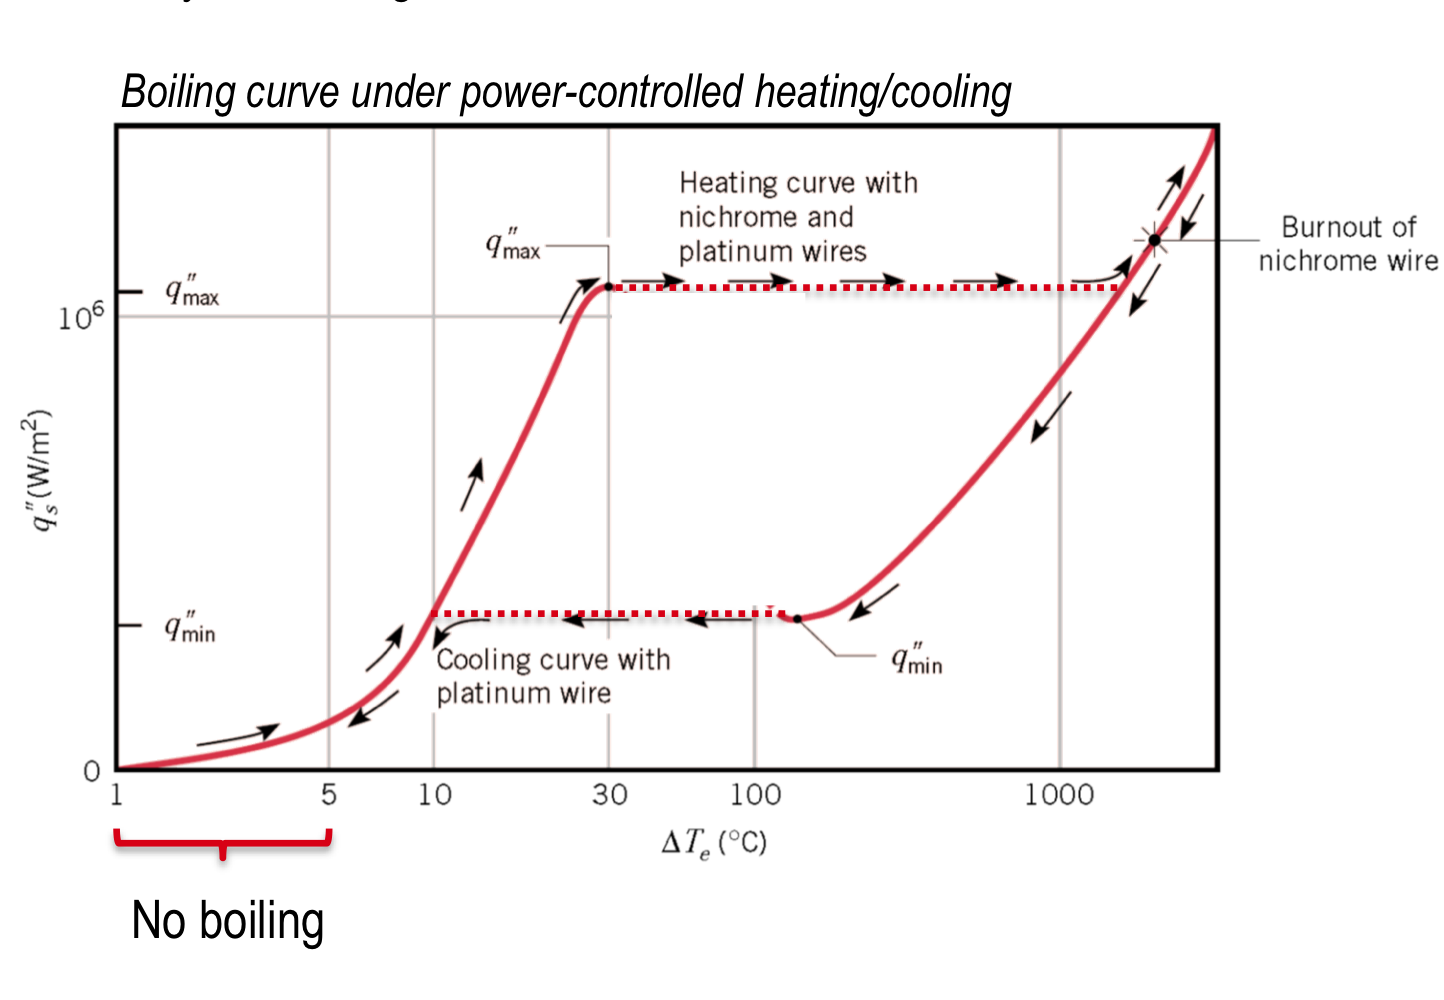
\includegraphics[width=.6\textwidth]{IMAGES/elec/PNG image.png}
\end{figure}

\subsubsection{Correlations}
Bubbles can be considered to cause forced convection. \\
\begin{itemize}
    \item Characteristic length : $D_b \propto \sqrt{\frac{\sigma}{g(\rho_1-\rho_2)}}$\\
    \item Characteristic velocity : $V \propto \frac{D_b}{t_b} \propto \frac{q_s"}{\rho_l h_{fg}}$\\
\end{itemize}

\begin{equation} \begin{gathered}
q_s" = \mu_l h_{fg} [\frac{g(\rho_l - \rho_v)}{\sigma}]^{1/2} (\frac{c_{p,l} \Delta T_e}{C_{s,f} h_{fg} Pr_l^n})^3\\
q_{max}"= Ch_{fg} \rho_v [\frac{\sigma g(\rho_l - \rho_v)}{\rho_v^2}]^{1/4}\\
q_{min}" = C \rho_v h_{fg} [\frac{g \sigma (\rho_l - \rho_v)}{(\rho_l + \rho_v)^2}]^{1/4}\\
\end{gathered}
\end{equation}

With : \begin{itemize}
\item $C = \frac{\pi}{24}$ for large horizontal cylinders, spheres, and finite heated surfaces\\
\item $C = 0.149$ for large horizontal plates\\
\end{itemize}

\subsubsection{Film Pool Boiling}
Happens when $\Delta T_e > 120^\circ C$\\

We have : \begin{equation}
    \overline{Nu}_D = C[\frac{g \rho_v (\rho_l-\rho_v) h'_{fg} D^3}{\mu_v \kappa_v (T_s-T_{sat})}]^{1/4}
\end{equation}

With $h'_{fg} = h_{fg} + 0.8 c_{pv} (T_s-T_{sat})$, $C = 0.62$ (horizontal cylinders), $C = 0.67$ for spheres.\\

With properties estimated at $T_f = \frac{T_s+T_{sat}}{2}$\\

if $T_s>300^\circ C$, we also have radiation : $\overline{h} = \overline{h}_{conv} + \frac{3}{4} \overline{h}_{rad}$\\

\subsubsection{Forced convection boiling}
Fluid is moving when boiling.\\

Two values for $q"_{max}$ possible, compute both and check validity : \begin{itemize}
    \item Low velocity : \begin{equation}
        \begin{gathered}
            \frac{q"_{max}}{\rho_v h_{fg} V} > [\frac{0.275}{\pi} (\frac{\rho_l}{\rho_v})^{1/2} + 1]\\
            \frac{q"_{max}}{\rho_v h_{fg} V} = \frac{1}{\pi} [1+(\frac{4}{We_d})^{1/3}]\\
        \end{gathered}
    \end{equation}
    \item High velocity : \begin{equation}
        \begin{gathered}
            \frac{q"_{max}}{\rho_v h_{fg} V} < [\frac{0.275}{\pi} (\frac{\rho_l}{\rho_v})^{1/2} + 1]\\
            \frac{q"_{max}}{\rho_v h_{fg} V} = \frac{(\frac{\rho_l}{\rho_v})^{3/4}}{169\pi} + \frac{(\frac{\rho_l}{\rho_v})^{1/2}}{19.2\pi We_D^{1/3}}\\
        \end{gathered}
    \end{equation}
\end{itemize}
Where $We_D = \frac{\rho_v V^2 D}{\sigma}$ and V the fluid velocity.\\

\subsubsection{Internal forced convection boiling}
Heat transfer coefficient is independent of the heat flux but depends on the velocity and quality factor. \\
\textbf{Vapor quality :} $X = \frac{\dot{m}_v}{\dot{m}_{tot}}$\\
With $G = \dot{m}_{tot}$, $G_l = (1-X)G$ and $G_g = XG$\\

We have seven phases : liquid forced convection, sub-cooled flow boiling, bubbly, slug, annular, mist, vapor forced convection.\\

For saturated flow boiling in smooth circular tubes (use largest h between the two) : \begin{equation}
    \begin{gathered}
        \frac{h}{h_{sp}} = 0.6683 (\frac{\rho_l}{\rho_v})^{0.1} \overline{X}^{0.16} (1-\overline{X})^{0.64} f(Fr) + 1058(\frac{q"_s}{\dot{m} h_{fg}})^{0.7} (1-\overline{X})^{0.8} G_{s,f}\\
        \frac{h}{h_{sp}} = 1.136 (\frac{\rho_l}{\rho_v})^{0.45} \overline{X}^{0.72} (1-\overline{X})^{0.08} f(Fr) + 667.2(\frac{q"_s}{\dot{m}h_{fg}})^{0.7} (1-\overline{X})^{0.8} G_{sf}\\
    \end{gathered}
\end{equation}

Where $\overline{X} = \frac{q"_s \pi Dx}{\dot{m} h_{fg}}$, and $\dot{m}" = \frac{\dot{m}}{A_c}$, $Fr = \frac{(\dot{m}"/\rho_l)^2}{gD}$\\

Also, $f(Fr) = 1$ (vertical and horizontal tubes $Fr>0.04$) and $f(Fr) = 2.63 Fr^{0.3}$ (horizontal tubes with $Fr<0.04$)\\

\subsubsection{Condensation}
Degradation of the surface properties can make the condensation go from drop-wise mode (better) to film mode (lower heat transfer rate)\\

We want to minimize the thickness of the condensate film.\\

From Fourier's law, we have $q"_s = \frac{\kappa_l (T_{sat}-T_s)}{\delta}$, with $\delta$ the condensate film thickness.\\

Also : $u(y) = \frac{g (\rho_l - \rho_v)\delta^2}{\mu_l} [\frac{y}{\delta} - \frac{1}{2} (\frac{y}{\delta})^2]$\\

Finally, we get $\delta(x) = [\frac{4\kappa_l \mu_l (T_{sat}-T_s)x}{g\rho_l (\rho_l - \rho_v) h'_{fg}}]^{1/4}$\\
$h'_{fg} = h_{fg} + 0.68c_{pl} (T_{sat}-T_s)$\\


\subsubsection{Film condensation}

We have the total condensation rate as : $\dot{m} = \frac{Q}{h_{fg}'} = \frac{\overline{h}_L A(T_{sat}-T_s)}{h_{fg}'}$\\

\quad \underline{Vertical plate correlations :}\\

We have : $Re_\delta = \frac{4\dot{m}}{\mu_l b} = \frac{4 \rho_l u_{mean} \delta}{\mu_l}$\\
And finally, $\overline{h}_L = \frac{Re_\delta \mu_l h_{fg}'}{4L (T_{sat}-T_s)}$\\

We have three relations possible for the $Re_\delta$ : \begin{itemize}
    \item $Re_\delta = 3.78 [\frac{\kappa_l L (T_{sat} - T_s)}{\mu_l h_{fg}' (\nu_l^2/g)^{1/3}}]^{3/4}$, $Re_\delta \leq 30$ (laminar)\\
    \item $Re_\delta = [\frac{3.7 \kappa_l L (T_{sat} - T_s)}{\mu_l h_{fg}' (\nu_l^2/g)^{1/3}} + 4.8]^{0.82}$, $30 \leq Re_\delta \leq 1800$ (wavy)\\
    \item $Re_\delta = [\frac{0.069 \kappa_l L (T_{sat} - T_s)}{\mu_l h_{fg}' (\nu_l^2/g)^{1/3}}Pr_l^{0.5} - 151 Pr_l^{0.5}+253]^{4/3}$, $Re_\delta \geq 1800$ (turbulent)\\
\end{itemize}

Where the liquid properties are estimated at $T_f = \frac{T_s + T_{sat}}{2}$\\

\quad \underline{Radial systems :}\\

\begin{itemize}
    \item Single tube : $\overline{h}_D = C[\frac{g \rho_l (\rho_l - \rho_v) \kappa_l^3 h_{fg}'}{\mu_l (T_{sat} - T_s)D}]^{1/4}$ \begin{itemize}
        \item $C = 0.862$ for a sphere\\
        \item $C = 0.729$ for a cylindrical tube\\
    \end{itemize}
    \item Bank of tubes : $\overline{h}_D = 0.729[\frac{g \rho_l (\rho_l - \rho_v) \kappa_l^3 h_{fg}'}{N \mu_l (T_{sat} - T_s)D}]^{1/4}$, N the number of tubes in a column\\
\end{itemize}

The condensed mass-flow rate per unit length of a single tube is : $\dot{m}_1' = \frac{\overline{h}_D \pi D (T_{sat}-T_s)}{h_{fg}'}$\\

The total heat transfer is equal to : $Q = \frac{T_{sat}-T_s}{R_{tot}}$\\

\subsection{Heat exchanger}
The most general formula is : (given we have fins inside and outside of the tubes) \begin{equation}
    \frac{1}{UA} = \frac{1}{\eta_{o,out} h_{out} A_{out}} + \frac{R_{f,o}"}{\eta_{o,out} A_{out}} + R_{cond} + \frac{R_{f,i}"}{\eta_{o,in} A_{in}} + \frac{1}{\eta_{o,in} h_{in} A_{in}}
\end{equation}

Where we take into account the fouling (rust and deposit on tubes after time).\\

\subsubsection{Concentric flow}

We denote $i$ the enthalpy.\\

\quad \underline{Parallel flow :}\\

From energy balance : $Q = Q_c = -Q_h = -\dot{m}_h c_{p,h} (T_{h,out} - T_{h,in}) = \dot{m}_c c_{p,c} (T_{c,out} - T_{c,in})$\\

Consider the fluid specific heat constant, overall heat transfer coefficient constant, we get : \begin{equation}
\begin{gathered}
    Q = UA \frac{\Delta T_2 - \Delta T_1}{\ln(\Delta T_2 / \Delta T_1)} = UA \Delta T_m\\
    \Delta T_m = \frac{\Delta T_2 - \Delta T_1}{\ln(\Delta T_2 / \Delta T_1)}\\
    \Delta T_1 = T_{h,1} - T_{c,1}\\
    \Delta T_2 = T_{h,2} - T_{c,2}\\
    \end{gathered}
\end{equation}

\quad \underline{Counter flow :}\\

We can exchange more energy by doing so as the temperature profile develops in a better way.\\

We get the same result : 
 \begin{equation}
\begin{gathered}
    Q = UA \frac{\Delta T_2 - \Delta T_1}{\ln(\Delta T_2 / \Delta T_1)} = UA \Delta T_m\\
    \Delta T_m = \frac{\Delta T_2 - \Delta T_1}{\ln(\Delta T_2 / \Delta T_1)}\\
    \Delta T_1 = T_{h,in} - T_{c,out}\\
    \Delta T_2 = T_{h,out} - T_{c,in}\\
    \end{gathered}
\end{equation}

\subsubsection{Effectiveness - NTU method}
We want to know $Q_{max}$. We therefore choose $\Delta T_{max}$ along with $C_{min} = \dot{m} c_p$\\

\begin{equation}
    \begin{gathered}
        Q_{max} = C_{min} \Delta T_{min}\\
        \varepsilon = \frac{Q}{Q_{max}} = \frac{C_h(T_{h,in} - T_{h,out})}{C_{min} (T_{h,in} - T_{c,in})} = \frac{C_c(T_{c,out} - T_{c,in})}{C_{min} (T_{h,in} - T_{c,in})}\\
        Q = \varepsilon C_{min} (T_{h,in} - T_{c,in})\\
        \varepsilon = NTU \frac{\Delta T_{lm}}{(T_{h,in} - T_{c,in})}\\
        NTU = \frac{UA}{C_{min}}\\
    \end{gathered}
\end{equation}
With NTU the number of heat transfer units. \\

For parallel flow heat exchanger, we have $\varepsilon = \frac{1-\exp(-NTU[1+ C_{min}/C_{max}])}{1+ C_{min}/C_{max}}$\\

\subsection{Radiation}

\subsubsection{Interaction of Thermal Radiation with matter}
We define here three variables : \begin{itemize}
    \item $\rho_\lambda$ the reflectivity\\
    \item $\tau_\lambda$ the transmissivity\\
    \item $\alpha_\lambda$ the absorptivity\\
\end{itemize}
$G_\lambda = G_{\lambda, abs} + G_{\lambda, ref} + G_{\lambda, tr}\Rightarrow 1 = \alpha_\lambda + \rho_\lambda + \tau_\lambda$\\

\subsubsection{Measures of radiation}
\begin{table}[hbt!]
    \centering
    \begin{tabular}{|c|c|c|c|}
    \hline
         & Intensity $I_{\lambda,x}$ & Spectral $X_\lambda(\lambda) = \int_0^{2\pi} \int_0^{\pi/2} I_{\lambda, x} (\lambda, \theta, \phi) \cos\theta \sin\theta d\phi d\theta$ & Total $X = \int_0^\infty X_\lambda (\lambda)d\lambda$ \\
         \hline
        Emission & $I_{\lambda,e}(\lambda, \theta, \phi)$ & $E_\lambda$ spectral emissive power & $E$ emissive power\\
        Irradiation & $I_{\lambda,i}(\lambda, \theta, \phi)$ & $G_\lambda$ spectral irradiation & $G$ irradiation\\
        Emission & $I_{\lambda,e+r}(\lambda, \theta, \phi)$ & $J_\lambda$ spectral radiosity & $J$ radiosity\\ \hline
    \end{tabular}
\end{table}
With the following relations : \begin{itemize}
    \item Diffuse emitter : $I_{\lambda, e} (\lambda, \theta, \phi) =I_{\lambda,e}(\lambda)$\\
    \item Diffuse irradiation : $I_{\lambda, i} (\lambda, \theta, \phi) =I_{\lambda,i}(\lambda)$\\
    \item Diffuse emitter and diffuse reflector : $I_{\lambda, e+r} (\lambda, \theta, \phi) =I_{\lambda,e+r}(\lambda)$\\
    \item In theses cases, we have $X_\lambda (\lambda) = \pi I_{\lambda, x}(\lambda)$\\
    \item $X = \pi I_x$\\
    \item $I_x = \int_0^\infty I_{\lambda, x}(\lambda) d\lambda$ the total intensity\\
\end{itemize}

A \textbf{diffuse emitter} is a surface that emits radiation at the same rate irrespective of the emission direction.

\subsubsection{Black body}
A black body is an object that for all wavelengths absorbs all the radiation ($\alpha_\lambda = 1$)\\

A black body is by definition a diffuse emitter [$\frac{W}{m^2 sr \mu m}$] : \begin{equation}
    I_{\lambda,b} = \frac{2hc_0^2}{\lambda^2 [\exp(h c_0/\lambda \kappa T) - 1]}
\end{equation}

With \begin{itemize}
    \item $h = 6.626 x 10^{-34} Js$ Planck constant\\
    \item $\kappa = 1.381 x 10^{-23} J/K$ Boltzmann constant\\
    \item $c_0 = 2.998x 10^8 m/s$ speed of light\\
\end{itemize}

We have Boltzman law : \begin{equation}\begin{gathered}
    E_b(T) = \sigma T^4\\
 '   \sigma = 5.67 10^{-8} W/m^2K^4\\
    I_b = \frac{E_b}{\pi}\\
    \end{gathered}
\end{equation}

From \textbf{Wien's Law} (peak emission), we have $(\lambda T)_{e_{\lambda=max}} = 2898 \mu m K$\\

We have $G_\lambda = G_{\lambda, abs} = E_{\lambda, b}$\\

\subsubsection{Real surfaces : emissivity}
We can describe the emission of real surfaces with respect to the ideal black body.

\begin{equation}
    \begin{gathered}
        E_\lambda(\lambda, T) = \varepsilon_\lambda E_{\lambda, b}(\lambda, T)\\
        I_\lambda (\lambda, \theta, \phi, T) = \varepsilon_{\lambda, b} I_{\lambda, b} (\lambda, T)\\
    \end{gathered}
\end{equation}

We have the relations : \begin{equation}
    \begin{gathered}
        \varepsilon_{\lambda, \theta} = \frac{I_\lambda (\lambda, \theta, \phi, T)}{I_{\lambda, b}(\lambda, T)}\\
        \varepsilon(T) = \frac{E(T)}{E_b(T)} = \frac{\int_0^\infty \varepsilon_\lambda (\lambda, T) E_{\lambda,b}(\lambda, T)d\lambda}{E_b(T)}\\
        E(T) = \varepsilon E_b(T) = \varepsilon \sigma T^4\\
    \end{gathered}
\end{equation}

Also define a function $F_{0\rightarrow a} = \frac{\int_0^a E_{\lambda,b}(\lambda, T)d\lambda}{\int_0^\infty E_{b,\lambda}(\lambda,T)d\lambda}$\\

For a real surface, we compute : \begin{itemize}
    \item $\alpha = \frac{G_{abs}}{G} = \frac{\int_0^\infty \alpha_\lambda G_\lambda d\lambda}{\int_0^\infty G_\lambda d\lambda}$\\
    \item $\rho = \frac{G_{ref}}{G} = \frac{\int_0^\infty \rho_\lambda G_\lambda d\lambda}{\int_0^\infty G_\lambda d\lambda}$\\
    \item $\tau = \frac{G_{tr}}{G} = \frac{\int_0^\infty \tau_\lambda G_\lambda d\lambda}{\int_0^\infty G_\lambda d\lambda}$\\
\end{itemize}

We typically assume that $G_\lambda$ can be replaced by $E_{\lambda, b}$ : $\alpha_\lambda G_\lambda = E_\lambda = G_{\lambda, abs} = \varepsilon_{\lambda} E_{\lambda,b}$.\\

\begin{itemize}
    \item Diffuse surface : $\varepsilon_{\lambda,\theta} = \varepsilon_\lambda$, $\alpha_{\alpha,\theta} = \alpha_\lambda$\\
    \item Gray surface : $\varepsilon_\lambda = \varepsilon$, $\alpha_\lambda = \alpha$\\
\end{itemize}

From Kirchoff's Laws, we have $\varepsilon_{\lambda,\theta} = \alpha_{\lambda,\theta}$.\\

\begin{itemize}
    \item If the irradiation is diffuse or if the surface is diffuse : $\varepsilon_\lambda = \alpha_\lambda$\\
    \item If the irradiation is a black body emission or the surface is gray : $\varepsilon = \alpha$\\
\end{itemize}

\subsubsection{View factor}
The view factor $F_{ij}$ is the fraction of the radiation leaving surface i that is intercepted by surface j.\\
\begin{equation}\begin{gathered}
    F_{ij} =  \frac{Q_{i-j}}{A_iJ_i} = \frac{1}{A_i} \int_{A_i} \int_{A_j} \frac{\cos \theta_i \cos\theta_j}{\pi R^2} dA_jdA_i\\
    A_i F_{ij} = A_j F_{ji}\\
    \end{gathered}
\end{equation}
\begin{itemize}
    \item If a surface is concave : $F_{ii} \neq 0$\\
    \item If a surface is convex : $F_{ii} = 0$\\
    \item In an enclosure $\sum_{j = 1}^N F_{ij} = 1$\\
\end{itemize}

\begin{equation}
    Q_i = A_i (J_i - \frac{J_i - \varepsilon_i E_b(T_i)}{\rho_i})
\end{equation}

If we consider an isothermal, opaque, diffuse and gray surface : \begin{equation}
    \begin{gathered}
        Q_i = \frac{E_b(T_i) - J_i}{R_{surf,rad}}\\
        R_{surf, rad} = \frac{1-\varepsilon_i}{\varepsilon_i A_i}\\
    \end{gathered}
\end{equation}

In a multi-surface enclosure, we have $Q_i = \sum_{j=1}^N \frac{J_i-J_j}{R_{geom, ij}}$\\




\end{document}